% The generic preamble
\documentclass[10pt,letterpaper,fleqn,titlepage]{article}

% Define packages to use
\usepackage{natbib}
\usepackage[dvips]{graphicx,color}
\usepackage{amsmath,amssymb}
\usepackage{bm}
\usepackage{caption}
\usepackage{xr}
\usepackage{ifthen}
\usepackage[dvipdfm,colorlinks,linkcolor=blue,citecolor=blue,urlcolor=blue]{hyperref}
\usepackage{fancybox}
\usepackage{textcomp}
\usepackage{alltt}
%\usepackage{floatflt}
%\usepackage{svn}


% Redefine default page
\setlength{\textheight}{9in}  % 1" above and below
\setlength{\textwidth}{6.75in}   % 0.5" left and right
\setlength{\oddsidemargin}{-0.25in}

% Redefine default paragraph
\setlength{\parindent}{0pt}
\setlength{\parskip}{1ex plus 0.5ex minus 0.2ex}

% Define caption width and default fonts
\setlength{\captionmargin}{0.5in}
\renewcommand{\captionfont}{\sffamily}
\renewcommand{\captionlabelfont}{\bfseries\sffamily}

% Define commands for super- and subscript in text mode
\newcommand{\superscript}[1]{\ensuremath{^\textrm{#1}}}
\newcommand{\subscript}[1]{\ensuremath{_\textrm{#1}}}

% Derived commands
\newcommand{\invcm}{\textrm{cm\superscript{-1}}}
\newcommand{\micron}{\ensuremath{\mu\textrm{m}}}

\newcommand{\df}{\ensuremath{\delta f}}
\newcommand{\Df}{\ensuremath{\Delta f}}
\newcommand{\dx}{\ensuremath{\delta x}}
\newcommand{\Dx}{\ensuremath{X_{max}}}
\newcommand{\Xeff}{\ensuremath{X_{eff}}}

\newcommand{\water}{\textrm{H\subscript{2}O}}
\newcommand{\carbondioxide}{\textrm{CO\subscript{2}}}
\newcommand{\ozone}{\textrm{O\subscript{3}}}

\newcommand{\taup}[1]{\ensuremath{\tau_{#1}}}
\newcommand{\efftaup}[1]{\ensuremath{\tau_{#1}^{*}}}

\newcommand{\textbfm}[1]{\boldmath\ensuremath{#1}\unboldmath}

\newcommand{\rb}[1]{\raisebox{1.5ex}[0pt]{#1}}

\newcommand{\f}[1]{\texttt{#1}}

% Define how equations are numbered
\numberwithin{equation}{section}
\numberwithin{figure}{section}
\numberwithin{table}{section}

% Define a command for title page author email footnote
\newcommand{\email}[1]
{%
  \renewcommand{\thefootnote}{\alph{footnote}}%
  \footnote{#1}
  \renewcommand{\thefootnote}{\arabic{footnote}}
}

% Define a command to print the Office Note subheading
\newcommand{\notesubheading}[1]
{%
  \ifthenelse{\equal{#1}{}}{}
  { {\Large\bfseries Office Note #1\par}%
    {\scriptsize \sc This is an unreviewed manuscript, primarily intended for informal}\\ 
    {\scriptsize \sc exchange of information among JCSDA researchers\par}%
  }
}

% Redefine the maketitle macro
\makeatletter
\def\docseries#1{\def\@docseries{#1}}
\def\docnumber#1{\def\@docnumber{#1}}
\renewcommand{\maketitle}
{%
  \thispagestyle{empty}
  \vspace*{1in}
  \begin{center}%
     \sffamily
     {\huge\bfseries Joint Center for Satellite Data Assimilation\par}%
     \notesubheading{\@docnumber}
  \end{center}
  \begin{flushleft}%
     \sffamily
     \vspace*{0.5in}
     {\Large\bfseries\ifthenelse{\equal{\@docseries}{}}{}{\@docseries: }\@title\par}%
     \medskip
     {\large\@author\par}%
     \medskip
     {\large\@date\par}%
     \bigskip\hrule\vspace*{2pc}%
  \end{flushleft}%
  \newpage
  \setcounter{footnote}{0}
}
\makeatother
\docseries{}
\docnumber{}


% Define a command for a DRAFT watermark
\usepackage{eso-pic}
\newcommand{\draftwatermark}
{
  \AddToShipoutPicture{%
    \definecolor{lightgray}{gray}{.85}
    \setlength{\unitlength}{1in}
    \put(2.5,3.5){%
      \rotatebox{45}{%
        \resizebox{4in}{1in}{%
          \textsf{\textcolor{lightgray}{DRAFT}}
        }
      }
    }
  }
}




% Define included documents
%\includeonly{}

% Title info
\title{Implementation of FASTEM-4 in the CRTM}
\author{Paul van Delst\footnote{paul.vandelst@noaa.gov}\\JCSDA/EMC/IMSG\\[0.25in]
        David N. Groff\footnote{david.groff@noaa.gov}\\JCSDA/EMC/IMSG.}
\date{April, 2011}
\docnumber{1}

%-------------------------------------------------------------------------------
%                            Ze document begins...
%-------------------------------------------------------------------------------
\begin{document}
\maketitle

%\draftwatermark

\section{Updating the CRTM's Incarnation of Fastem4 to be Consistent With What is Used in RTTOV}


\section{Radiometric Impact of Implementing FASTEM-4 into the CRTM}
The radiometric impact of implementing FASTEM-4 for any particular CRTM simulation depends on the channel central frequency, sensor zenith angle, salinity, sea-surface temperature, surface wind speed and the angle between the wind direction and the sensor azimuth angle.  For a standard tropical atmosphere we performed CRTM simulations using FASTEM-4 and the MWSSEM that was used in CRTM release 2.0.2 for NOAA-19 AMSUA, NOAA-19 MHS, F16 SSMIS and Aqua AMSRE to assess how the magnitude of the radiometric impact depends on these inputs.  CRTM simulations for release 2.0.2 were based on the 'Low Frequency' model for channel frequencies less than 20 GHz and FASTEM1 for channel frequencies greater than 20 GHz. 

\subsection{Dependance on Channel Frequency}
The channel central frequency determines the sensitivity to the surface.  As such the radiometric impact resulting from emissivity differences depends strongly on the channel central frequency.  For example as shown in figure \ref{fig:AMSUA_Wind_Speed_Impact} the magnitude of the impact on simulations for AMSUA NOAA-19 surface channels can be more than 5K depending on the wind speed; whereas for some of the high peaking channels the impact is neglibible regardless of the wind speed.  The CRTM release 2.0.2 microwave sea surface emissivities for all AMSUA surface sensitive channels are computed based on the Fastem-1 model.

\subsection{Dependence on Sensor Zenith Angle}
For AMSRE Aqua channels 1-4 the CRTM brightness temperatures using FASTEM-4 are larger than those when using the CRTM's release 2.0.2 microwave sea surface emissivities with the exception of cases where the sensor zenith angles exceed 60.  The smaller CRTM brightness temperatures when using Fastem-4 for large sensor zenith angles is due to the exponential inverse relationship between the cosine of the sensor zenith angle and the small scale correction.  For AMSRE Aqua channels 1-6 the CRTM release 2.0.2 emissivities were computed using the 'Low Frequency' microwave sea surface emissivity model.  Figure \ref{fig:AMSRE_Sensor_Zenith_Impact} shows that CRTM brightness temperature simulations for AMSRE Aqua channels using FASTEM-4 can be significantly smaller than those when using the CRTM release 2.0.2 microwave sea surface emissivities for angles larger than 60.  

\begin{figure}[htp]
  \centering
  \includegraphics[scale=0.75]{graphics/AMSUA_Wind_Speed_BT.eps}
  \caption{The radiometric impact of implementing FASTEM-4 on AMSUA NOAA-19 simulations as a function of wind speed.}
  \label{fig:AMSUA_Wind_Speed_Impact}
\end{figure}

\newpage

\begin{figure}[htp]
  \centering
  \includegraphics[scale=0.75]{graphics/AMSRE_Sensor_Zenith_BT.eps}
  \caption{The radiometric impact of implementing FASTEM-4 on AMSRE Aqua simulations as a function of sensor zenith angle.}
  \label{fig:AMSRE_Sensor_Zenith_Impact}
\end{figure}

\begin{figure}[htp]
  \centering
  \includegraphics[scale=0.75]{graphics/AMSRE_Wind_Speed_BT.eps}
  \caption{The radiometric impact of implementing FASTEM-4 on AMSRE Aqua simulations as a function of wind speed.}
  \label{fig:AMSRE_Wind_Speed_Impact}
\end{figure}

%\newpage

\subsection{Dependence on Wind Speed}
The impact on CRTM simulations for any particular surface sensitive microwave channel is strongly dependent on the surface wind speed.  The maximum impact on CRTM simulations as a function of wind speed occurs at around 10 m/s.  Figure \ref{fig:AMSUA_Wind_Speed_Impact} shows that among the 4 most surface sensitive AMSUA channels the magnitude of the impact for the range of wind speeds we considered can vary by as much as 4K.  

\begin{figure}[htp]
  \centering
  \includegraphics[scale=0.75]{graphics/emissD_windS_f.eps}
  \caption{The radiometric impact on MetOP-A AMSUA simulations as a function of wind speed using global NCEP background data from February 2, 2009 and August 1, 2009 as input.}
  \label{fig:AMSUA_Background_Impact}
\end{figure}

\newpage

\subsection{Dependence on Salinity}
The impact on CRTM simulations is much less dependent on salinity than wind speed.  Figure \ref{fig:AMSUA_Salinity_Impact} shows that among the 4 most surface sensitive AMSUA channels the magnitude of the impact varies by no more than about 1K.



  

\begin{figure}[htp]
  \centering
  \includegraphics[scale=0.75]{graphics/AMSUA_Salinity_BT.eps}
  \caption{The radiometric impact of implementing FASTEM-4 on AMSUA NOAA-19 simulations as a function of salinity.}
  \label{fig:AMSUA_Salinity_Impact}
\end{figure}

\begin{figure}[htp]
  \centering
  \includegraphics[scale=0.75]{graphics/MHS_Salinity_BT.eps}
  \caption{The radiometric impact of implementing FASTEM-4 on MHS NOAA-19 simulations as a function of salinity.}
  \label{fig:MHS_Salinity_Impact}
\end{figure}

\newpage  

\subsection{Dependence on the Angle Between the Sensor Azimuth and Wind Direction} 
The impact increases or decreases with the perpendicularity of the sensor azimuth to the wind direction depending on the channel polarization.  For vertically polarized channels the impact increases with perpendicularity of the sensor azimuth to the wind direction; whereas for horizontally polarized channels the impact decreases with perpendicularity of the sensor azimuth to the wind direction.  Among the four most surface sensitive AMSUA NOAA-19 channels the impact can vary by as much as 1K as shown in figure \ref{fig:AMSUA_Sensor_Azimuth_Impact}.
  

\begin{figure}[htp]
  \centering
  \includegraphics[scale=0.75]{graphics/AMSUA_Sensor_Azimuth_BT.eps}
  \caption{The radiometric impact of implementing FASTEM-4 as a function of the angle between the wind direction and sensor azimuth.}
  \label{fig:AMSUA_Sensor_Azimuth_Impact}
\end{figure} 

% The references section
%=======================
%\clearpage
%\bibliographystyle{plainnat}
%\bibliography{bibliography}
%\begin{thebibliography}{99}
%  \bibitem{ref:tag1} reference1
%  \bibitem{ref:tag2} reference2
%\end{thebibliography}

% The appendices section
%=======================
%\begin{appendix}
%\end{appendix}

\end{document}
